\documentclass[aspectratio=169,9pt]{beamer}

\usepackage{fontspec}
\usepackage[spanish]{babel}
\usepackage{graphicx}
\usepackage{tikz}
\usetikzlibrary{positioning,arrows.meta}
\usepackage{booktabs}
\usepackage{xcolor}

\setsansfont{PlusJakartaSans-Regular.ttf}[
  Path = fuentes/,
  BoldFont = PlusJakartaSans-Bold.ttf,
  ItalicFont = PlusJakartaSans-Regular.ttf,
  BoldItalicFont = PlusJakartaSans-Bold.ttf
]
\setmainfont{PlusJakartaSans-Regular.ttf}[
  Path = fuentes/,
  BoldFont = PlusJakartaSans-Bold.ttf,
  ItalicFont = PlusJakartaSans-Regular.ttf,
  BoldItalicFont = PlusJakartaSans-Bold.ttf
]
\newfontfamily\njsemibold{PlusJakartaSans-SemiBold.ttf}[Path=fuentes/]
\newfontfamily\njextrabold{PlusJakartaSans-ExtraBold.ttf}[Path=fuentes/]

\definecolor{ink}{HTML}{10231F}
\definecolor{cream}{HTML}{F7F3EB}
\definecolor{paper}{HTML}{FFFDF8}
\definecolor{tide}{HTML}{0F6B63}
\definecolor{tidedeep}{HTML}{0A4A40}
\definecolor{brick}{HTML}{C41E3A}
\definecolor{ember}{HTML}{E86A2A}
\definecolor{sand}{HTML}{E6DFD3}
\definecolor{mute}{HTML}{5E6864}

\setbeamercolor{background canvas}{bg=cream}
\setbeamercolor{normal text}{fg=ink,bg=cream}
\setbeamercolor{frametitle}{fg=ink,bg=cream}
\setbeamercolor{footline}{fg=mute,bg=cream}
\setbeamerfont{frametitle}{family=\njextrabold,size=\large}
\setbeamertemplate{navigation symbols}{}
\setbeamertemplate{headline}{}
\setbeamersize{text margin left=5.5mm,text margin right=5.5mm}
\setbeamertemplate{frametitle}{%
  \vspace{-1.2mm}%
  {\color{tide}\scriptsize\njsemibold\insertframenumber\hspace{1.6mm}\insertshorttitle}\par\vspace{0.6mm}%
  {\njextrabold\large\insertframetitle}\par\vspace{1.2mm}%
}
\setbeamertemplate{footline}{%
  \hspace{5.5mm}{\scriptsize\color{mute}NutriMatch · Paola Castañeda · corte del 2 de octubre de 2026}%
  \hfill{\scriptsize\color{tide}\insertframenumber\,/\,12}\hspace{5.5mm}\vspace{1.6mm}%
}

\newcommand{\metric}[1]{{\njextrabold\color{tidedeep}#1}}
\newcommand{\fine}[1]{{\scriptsize\color{mute}#1}}

\newcommand{\card}[2]{%
  \noindent\begin{tikzpicture}
    \node[draw=sand,line width=0.5pt,fill=paper,rounded corners=2.2mm,
          inner xsep=1.8mm,inner ysep=1.4mm,
          text width=\dimexpr#1-4.6mm\relax,align=left] {#2};
  \end{tikzpicture}%
}

\title{NutriMatch}
\subtitle{Defensa final}

\begin{document}

% ---------- 1 ----------
\begin{frame}[plain]
  \vspace{2mm}
  \begin{columns}[T]
    \begin{column}{0.58\textwidth}
      \begin{tikzpicture}
        \node[fill=tide,rounded corners=1.6mm,minimum width=7mm,minimum height=7mm,inner sep=0] (m) {};
        \draw[ember,line width=0.7pt] ([xshift=-2.1mm,yshift=0.4mm]m.center) .. controls ([xshift=-0.4mm,yshift=2.2mm]m.center) and ([xshift=0.6mm,yshift=2.2mm]m.center) .. ([xshift=2.2mm,yshift=0.4mm]m.center);
        \draw[paper,line width=1.15pt,line cap=round] ([xshift=-1.5mm,yshift=0.2mm]m.center) -- ([xshift=-0.2mm,yshift=-1.3mm]m.center) -- ([xshift=1.8mm,yshift=1.5mm]m.center);
        \fill[brick] ([xshift=-1.5mm,yshift=0.2mm]m.center) circle (0.55mm);
        \node[anchor=west,inner sep=0] at ([xshift=2.2mm]m.east) {{\njextrabold\color{tide}Nutri}{\njsemibold\color{ink}Match}};
      \end{tikzpicture}

      \vspace{5mm}
      {\color{tide}\scriptsize\njsemibold DIPLOMADO EN CIENCIA DE DATOS}\\[1.5mm]
      {\njextrabold\fontsize{28}{30}\selectfont NutriMatch}\\[2.5mm]
      {\njsemibold\large Sistema de apoyo a la decisión para la compra de alimentos empacados}\\[3mm]
      {\color{mute} De un catálogo heterogéneo a una decisión comprensible.}\\[5mm]
      {\njsemibold Paola Castañeda}\\
      {\scriptsize\color{mute}3 de octubre de 2026 · corte del catálogo: 2 de octubre de 2026}
    \end{column}
    \begin{column}{0.40\textwidth}
      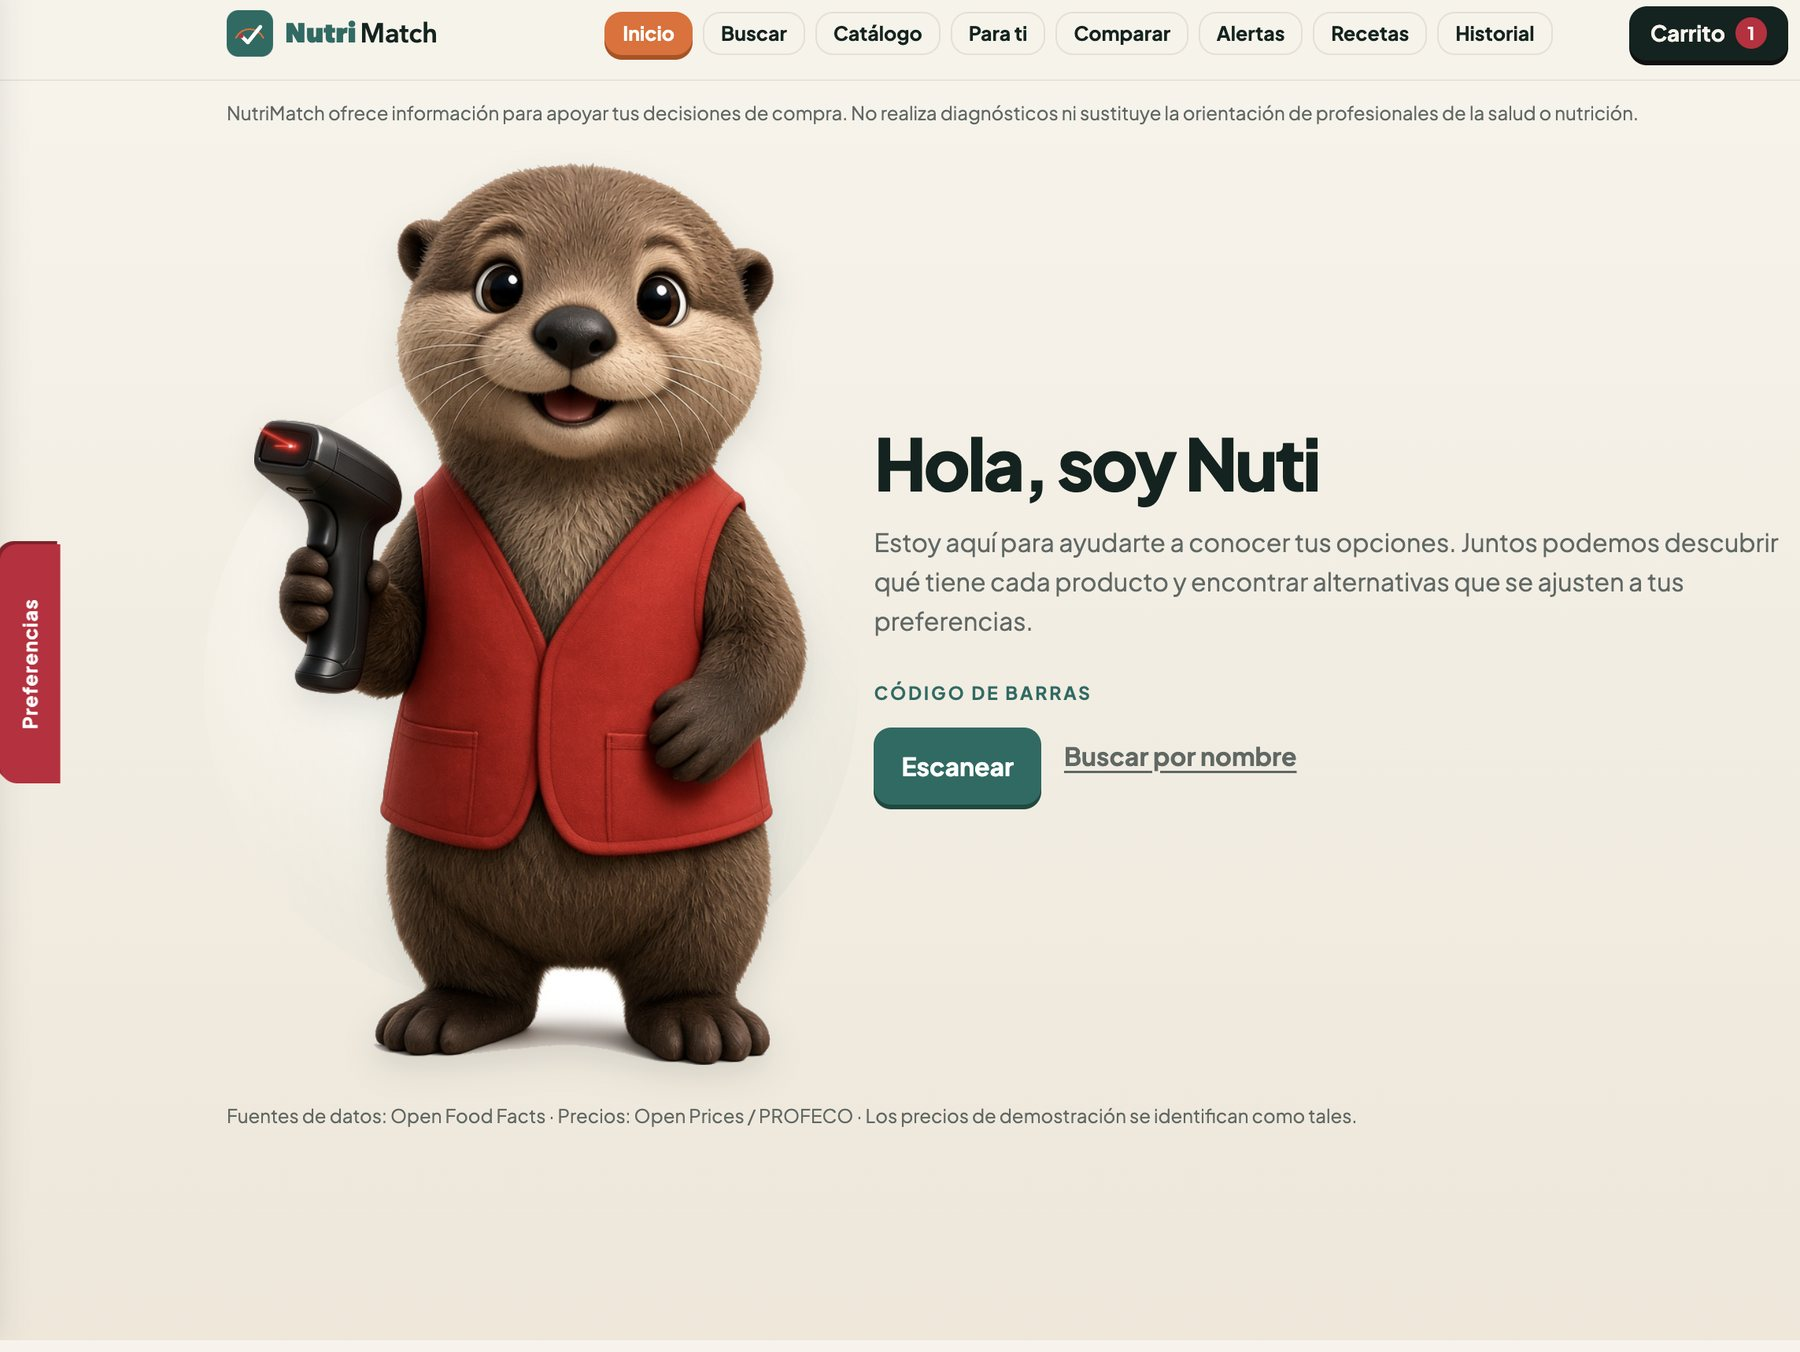
\includegraphics[width=\linewidth,height=62mm,keepaspectratio]{capturas/buscar.jpg}\\[1mm]
      {\scriptsize\color{mute}Inicio de la aplicación. La búsqueda abre la ficha del código.}
    \end{column}
  \end{columns}
\end{frame}

% ---------- 2 ----------
\begin{frame}{Elegir un alimento implica integrar información dispersa}
  \begin{columns}[T]
    \begin{column}{0.46\textwidth}
      \resizebox{0.96\linewidth}{!}{%
      \begin{tikzpicture}[pill/.style={draw=sand,fill=paper,rounded corners=1.3mm,inner xsep=1.6mm,inner ysep=1.2mm,font=\scriptsize}]
        \node[pill] at (0,0.95) {Nutrición};
        \node[pill] at (2.35,0.95) {Procesamiento};
        \node[pill] at (4.55,0.95) {Etiquetas};
        \node[pill,draw=tide,line width=0.7pt,font=\scriptsize\njsemibold] at (2.35,0) {Producto};
        \node[pill] at (0,-0.95) {Alérgenos};
        \node[pill] at (2.35,-0.95) {Precio};
        \node[pill,draw=ember] at (4.55,-0.95) {Faltante};
      \end{tikzpicture}}\par\vspace{1.6mm}
      \card{0.92\linewidth}{%
        {\njsemibold\color{brick} Si el faltante se trata como cero}\\
        {\scriptsize esa señal entra como el peor valor y el orden premia el silencio del registro.}\\[1.2mm]
        {\njsemibold\color{tide} Si el faltante se conserva}\\
        {\scriptsize esa señal no entra al promedio. Si la cobertura baja de 0,5, no hay puntaje.}%
      }
    \end{column}
    \begin{column}{0.52\textwidth}
      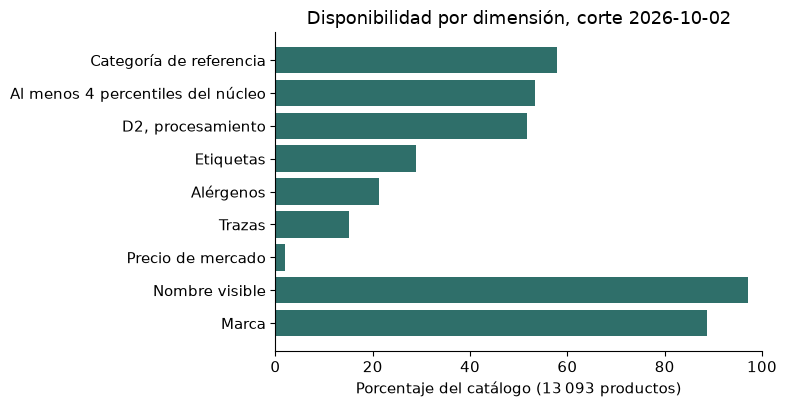
\includegraphics[width=\linewidth,height=58mm,keepaspectratio]{../documento_final/figuras/disponibilidad.png}\\[1mm]
      {\scriptsize Un dato ausente no es un cero.}\\
      {\fine{Figura del cuaderno. Precio, trazas y alérgenos cubren mucho menos que el nombre.}}
    \end{column}
  \end{columns}
\end{frame}

% ---------- 3 ----------
\begin{frame}{NutriMatch convierte información heterogénea en una decisión explicable}
  \centering
  \resizebox{0.98\textwidth}{!}{\begin{tikzpicture}[
    box/.style={draw=sand,fill=paper,rounded corners=1.6mm,inner xsep=1.3mm,inner ysep=1.8mm,
                text width=18mm,align=center,font=\scriptsize\njsemibold,minimum height=12mm},
    arr/.style={-{Stealth[length=1.6mm]},tide,line width=0.7pt}
  ]
    \node[box] (a) {Persona};
    \node[box,right=1.6mm of a] (b) {Prioridades};
    \node[box,right=1.6mm of b] (c) {Catálogo};
    \node[box,right=1.6mm of c] (d) {Preparación};
    \node[box,right=1.6mm of d,draw=tide] (e) {Motor};
    \node[box,right=1.6mm of e] (f) {Alternativas};
    \node[box,right=1.6mm of f] (g) {Carrito y alertas};
    \draw[arr] (a) -- (b);
    \draw[arr] (b) -- (c);
    \draw[arr] (c) -- (d);
    \draw[arr] (d) -- (e);
    \draw[arr] (e) -- (f);
    \draw[arr] (f) -- (g);
  \end{tikzpicture}}

  \vspace{2.5mm}
  \begin{columns}[T]
    \begin{column}{0.48\textwidth}
      \card{\linewidth}{%
        {\scriptsize La persona declara el orden de tres prioridades y, si quiere, dieta y alérgenos. No hay usuarias observadas.}\\[1.4mm]
        {\scriptsize El sistema busca el producto, lo evalúa con la información disponible y muestra alternativas de la misma categoría. Ella se queda, sustituye o revisa las alertas.}\\[1.4mm]
        {\scriptsize\color{tide}\njsemibold Apoya la decisión. No diagnostica y no determina si un alimento es saludable.}%
      }
    \end{column}
    \begin{column}{0.50\textwidth}
      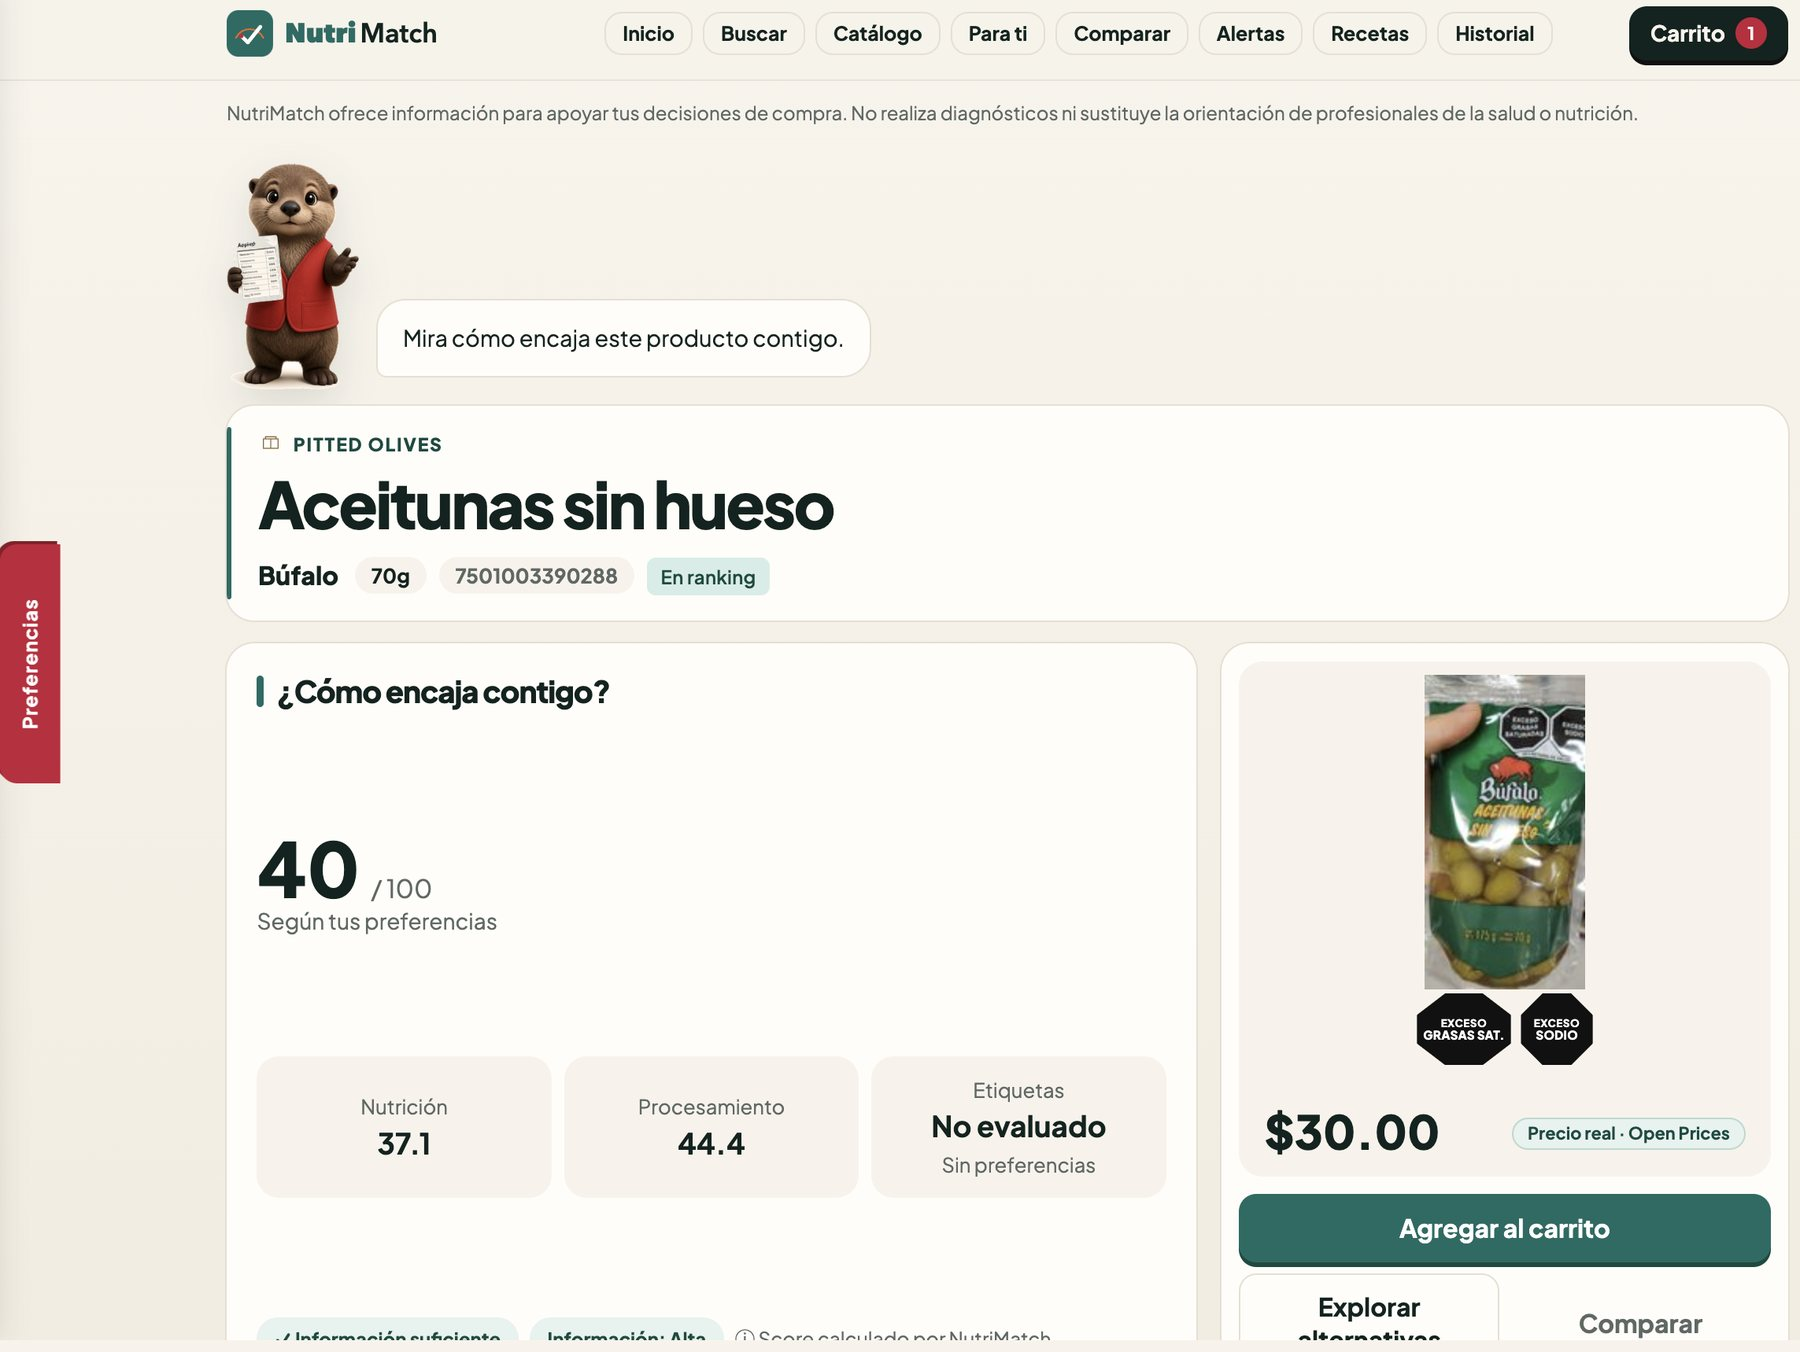
\includegraphics[width=\linewidth,height=42mm,keepaspectratio]{capturas/ficha-bufalo.jpg}\\[0.6mm]
      {\fine{Ficha real. En pantalla las dimensiones se llaman nutrición, procesamiento y etiquetas.}}
    \end{column}
  \end{columns}
\end{frame}

% ---------- 4 ----------
\begin{frame}{El reto comienza con la integración de fuentes}
  \begin{columns}[T]
    \begin{column}{0.34\textwidth}
      \card{\linewidth}{{\scriptsize\color{tide}\njsemibold Open Food Facts}\\{\scriptsize Ficha del producto: nutrientes, categoría, ingredientes, NOVA, etiquetas y alérgenos.}}\\[1.4mm]
      \card{\linewidth}{{\scriptsize\color{tide}\njsemibold Open Prices}\\{\scriptsize Precio en pesos por coincidencia exacta del código. 239 precios.}}\\[1.4mm]
      \card{\linewidth}{{\scriptsize\color{tide}\njsemibold PROFECO}\\{\scriptsize Precio solo si la coincidencia por texto quedó revisada. 20 precios.}}
    \end{column}
    \begin{column}{0.64\textwidth}
      \begin{columns}[c]
        \begin{column}{0.42\linewidth}
          {\scriptsize\color{mute} Filtro de México}\\[-0.5mm]
          {\metric{\fontsize{18}{20}\selectfont 16\,851}}\\[-1mm]
          {\scriptsize\color{mute} punto de partida}\\[1mm]
          {\color{tide}\njsemibold ↓\ tres candados}\\[1mm]
          {\scriptsize\color{mute} Catálogo oficial}\\[-0.5mm]
          {\metric{\fontsize{18}{20}\selectfont 13\,093}}
        \end{column}
        \begin{column}{0.56\linewidth}
          {\scriptsize
          \begin{tabular}{@{}r l@{}}
            −3 & no alimentarios → 16\,848 \\
            −3\,737 & integridad de identidad y nutrición → 13\,111 \\
            −18 & identidad del nombre → 13\,093 \\
          \end{tabular}}\\[2mm]
          {\metric{273}} {\scriptsize columnas \quad} {\metric{0}} {\scriptsize códigos duplicados}
        \end{column}
      \end{columns}
      \vspace{1.5mm}
      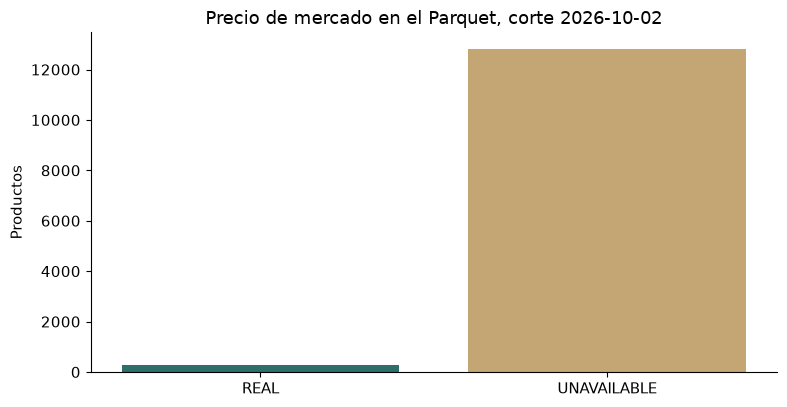
\includegraphics[width=0.62\linewidth,height=28mm,keepaspectratio]{../documento_final/figuras/precios.png}\\[1mm]
      {\fine{El filtro inicial de México no es todavía el universo evaluable. En el archivo hay 259 precios reales y 12\,834 sin precio. Cero imputados y cero sintéticos.}}
    \end{column}
  \end{columns}
\end{frame}

% ---------- 5 ----------
\begin{frame}{No todo el catálogo puede evaluarse de la misma manera}
  \begin{columns}[T]
    \begin{column}{0.62\textwidth}
      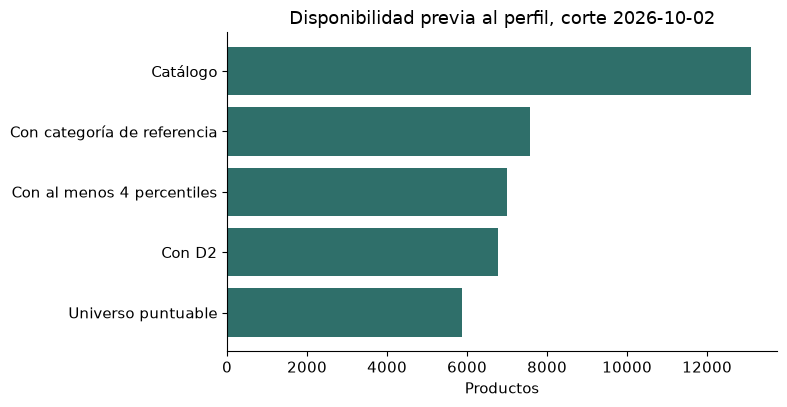
\includegraphics[width=\linewidth,height=62mm,keepaspectratio]{../documento_final/figuras/universo.png}
    \end{column}
    \begin{column}{0.36\textwidth}
      {\metric{\fontsize{22}{24}\selectfont 5\,864}}\\[-1mm]
      {\njsemibold\color{tide} 44,79\,\% del catálogo}\\[2mm]
      {\scriptsize Universo puntuable = procesamiento disponible y al menos 4 de 8 percentiles del núcleo.}\\[2mm]
      {\scriptsize Es la intersección de esas dos condiciones. Las barras de al lado miden coberturas por separado.}\\[2mm]
      \card{\linewidth}{{\scriptsize\njsemibold El universo puntuable no significa productos recomendados.} {\scriptsize Es el conjunto con información suficiente para aplicar esas dimensiones, antes de conocer a la persona.}}
    \end{column}
  \end{columns}
\end{frame}

% ---------- 6 ----------
\begin{frame}{De atributos del producto a dimensiones comparables}
  \begin{columns}[T]
    \begin{column}{0.32\textwidth}
      \card{\linewidth}{%
        {\scriptsize\color{tide}\njsemibold D1 · Nutrición}\\
        {\scriptsize Azúcares, sal y grasa saturada: menos es mejor.\\ Fibra y proteína: más es mejor.}\\[0.8mm]
        {\fine{Percentil dentro de la categoría de referencia, en escala 0–100.}}%
      }
    \end{column}
    \begin{column}{0.32\textwidth}
      \card{\linewidth}{%
        {\scriptsize\color{tide}\njsemibold D2 · Procesamiento}\\
        {\scriptsize Grupo NOVA en una banda de 25 puntos. Los aditivos empujan hacia el piso de la banda.}\\[0.8mm]
        {\fine{Sin grupo NOVA, esta dimensión no se calcula.}}%
      }
    \end{column}
    \begin{column}{0.32\textwidth}
      \card{\linewidth}{%
        {\scriptsize\color{tide}\njsemibold D3 · Preferencias}\\
        {\scriptsize Proporción de las etiquetas que la persona valora y el producto presenta.}\\[0.8mm]
        {\fine{Si no hay etiquetas que comparar, la dimensión queda vacía.}}%
      }
    \end{column}
  \end{columns}
  \vspace{1.6mm}
  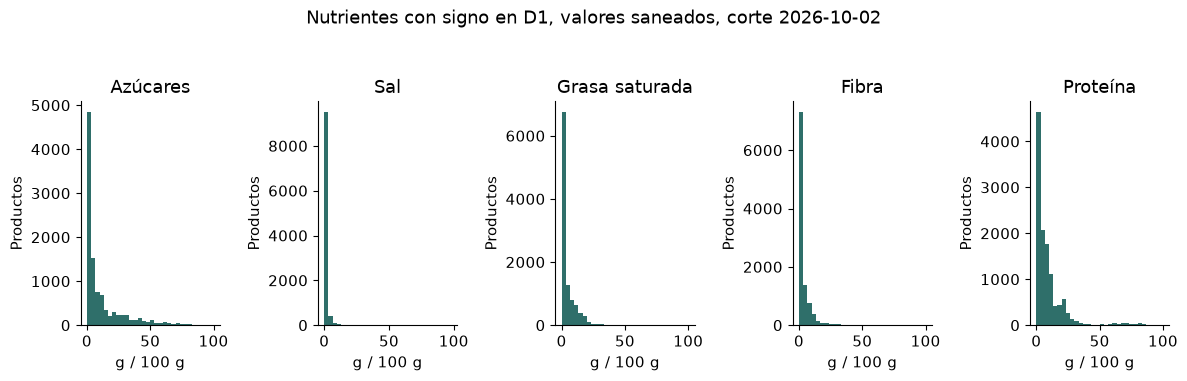
\includegraphics[width=0.78\textwidth,height=34mm,keepaspectratio]{../documento_final/figuras/nutrientes_d1.png}\\[0.4mm]
  {\fine{Las distribuciones están concentradas cerca de cero. Por eso la comparación es el percentil dentro de la categoría, no los gramos crudos. No se imputaron nutrientes, alérgenos, etiquetas, NOVA ni precio.}}
\end{frame}

% ---------- 7 ----------
\begin{frame}{Un motor determinista que respeta la información disponible}
  \begin{columns}[T]
    \begin{column}{0.58\textwidth}
      {\scriptsize Ejemplo de orden declarado: nutrición, preferencias, procesamiento.}\\[1mm]
      \resizebox{\linewidth}{!}{%
      \begin{tikzpicture}
        \node[fill=tide,text=white,rounded corners=1.5mm,minimum width=32mm,minimum height=13mm,font=\scriptsize,align=center] {Prioridad 1\\ \njextrabold 50\,\%};
        \node[fill=tide!75!white,text=white,rounded corners=1.5mm,minimum width=32mm,minimum height=13mm,font=\scriptsize,align=center] at (3.6,0) {Prioridad 2\\ \njextrabold 33,3\,\%};
        \node[fill=tide!50!white,text=ink,rounded corners=1.5mm,minimum width=32mm,minimum height=13mm,font=\scriptsize,align=center] at (7.2,0) {Prioridad 3\\ \njextrabold 16,7\,\%};
      \end{tikzpicture}}\\[1.4mm]
      {\njextrabold\color{brick} Pesos declarados, no aprendidos.}\\[1.6mm]
      {\scriptsize
      \[
        s=\frac{\sum_{d\in A} w_d\, s_d}{\sum_{d\in A} w_d}
        \quad\text{si }\sum_{d\in A} w_d \ge 0{,}5
      \]
      }%
      {\fine{$A$ son las dimensiones con dato. Un faltante no entra como cero. Si la cobertura queda bajo 0,5, no hay puntaje.}}
    \end{column}
    \begin{column}{0.40\textwidth}
      {\scriptsize\njsemibold Una sola banda, en este orden}\\[1mm]
      \card{\linewidth}{{\scriptsize 1.\ Excluido}\\{\fine{Alergia no apta o dieta incompatible.}}}\\[1mm]
      \card{\linewidth}{{\scriptsize 2.\ No verificable}\\{\fine{Falta evidencia de alergia o de dieta.}}}\\[1mm]
      \card{\linewidth}{{\scriptsize 3.\ Información insuficiente}\\{\fine{Cobertura menor que 0,5.}}}\\[1mm]
      \card{\linewidth}{{\scriptsize 4.\ Ranking}\\{\fine{El resto, de mayor a menor resultado.}}}\\[1.4mm]
      {\fine{Nutri-Score, sellos y precio se muestran. No forman parte del puntaje.}}
    \end{column}
  \end{columns}
\end{frame}

% ---------- 8 ----------
\begin{frame}{¿Por qué no se entrenó un modelo supervisado?}
  \begin{columns}[T]
    \begin{column}{0.42\textwidth}
      \card{\linewidth}{{\scriptsize Catálogo publicado}}\\[-0.4mm]
      {\color{tide}\scriptsize\quad ↓}\\[-0.6mm]
      \card{\linewidth}{{\scriptsize No hay compras, clics, favoritos ni conversiones.}}\\[-0.4mm]
      {\color{tide}\scriptsize\quad ↓}\\[-0.6mm]
      \card{\linewidth}{{\scriptsize\njsemibold No existe un target observado.}}\\[-0.4mm]
      {\color{tide}\scriptsize\quad ↓}\\[-0.6mm]
      \card{\linewidth}{{\scriptsize Entrenar con el puntaje, o con D1, D2 y D3, sería circular.}}\\[-0.4mm]
      {\color{tide}\scriptsize\quad ↓}\\[-0.6mm]
      \card{\linewidth}{{\scriptsize\njsemibold Motor determinista y evaluación externa.}}
    \end{column}
    \begin{column}{0.56\textwidth}
      \begin{columns}[T]
        \begin{column}{0.42\linewidth}
          {\metric{\fontsize{16}{18}\selectfont 12\,/\,13}}\\
          {\fine{casos revisados a mano. El restante difiere en el nombre, no en el puntaje.}}
        \end{column}
        \begin{column}{0.56\linewidth}
          {\metric{\fontsize{16}{18}\selectfont −0,475683}}\\
          {\fine{Spearman, n = 6\,035. Contraste con Nutri-Score. No es ground truth ni el target.}}
        \end{column}
      \end{columns}
      \vspace{1mm}
      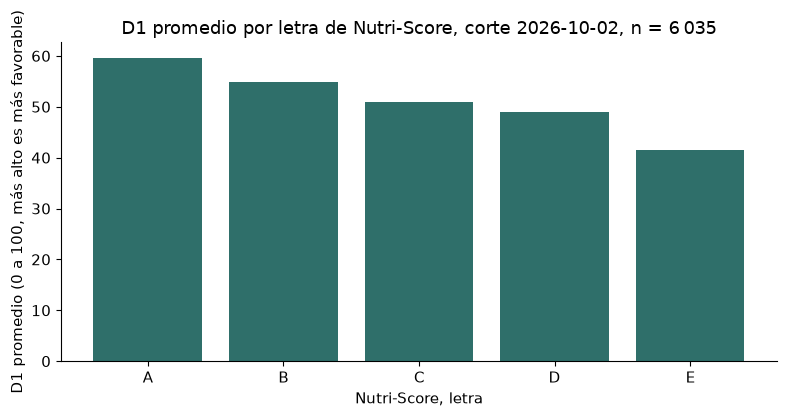
\includegraphics[width=\linewidth,height=36mm,keepaspectratio]{../documento_final/figuras/d1_nutriscore.png}\\[0.4mm]
      {\scriptsize A 59,68 \quad B 54,80 \quad C 50,87 \quad D 49,00 \quad E 41,57}\\
      {\fine{El signo negativo es esperable: aquí un valor alto es mejor y en Nutri-Score un valor alto es peor.}}
    \end{column}
  \end{columns}
\end{frame}

% ---------- 9 ----------
\begin{frame}{El mismo motor llega hasta la interfaz}
  \begin{columns}[T]
    \begin{column}{0.46\textwidth}
      \centering
      \begin{tikzpicture}[
        box/.style={draw=sand,fill=paper,rounded corners=1.6mm,minimum width=42mm,minimum height=7.2mm,font=\scriptsize\njsemibold},
        arr/.style={-{Stealth[length=1.5mm]},tide,line width=0.7pt}
      ]
        \node[box] (p) {Parquet};
        \node[box,below=2.2mm of p] (f) {Catálogo y variables};
        \node[box,below=2.2mm of f,draw=tide] (e) {Engine};
        \node[box,below=2.2mm of e] (a) {FastAPI};
        \node[box,below=2.2mm of a] (g) {Angular};
        \draw[arr] (p) -- (f);
        \draw[arr] (f) -- (e);
        \draw[arr] (e) -- (a);
        \draw[arr] (a) -- (g);
      \end{tikzpicture}\\[1.5mm]
      {\scriptsize
      \begin{tabular}{@{}l l@{}}
        Cuaderno & análisis y reproducibilidad \\
        Engine & la decisión \\
        API & el servicio \\
        Angular & la interacción \\
      \end{tabular}}\\[1mm]
      {\fine{La misma función puntúa en el cuaderno y en la aplicación. Angular no vuelve a calcular las tres dimensiones.}}
    \end{column}
    \begin{column}{0.52\textwidth}
      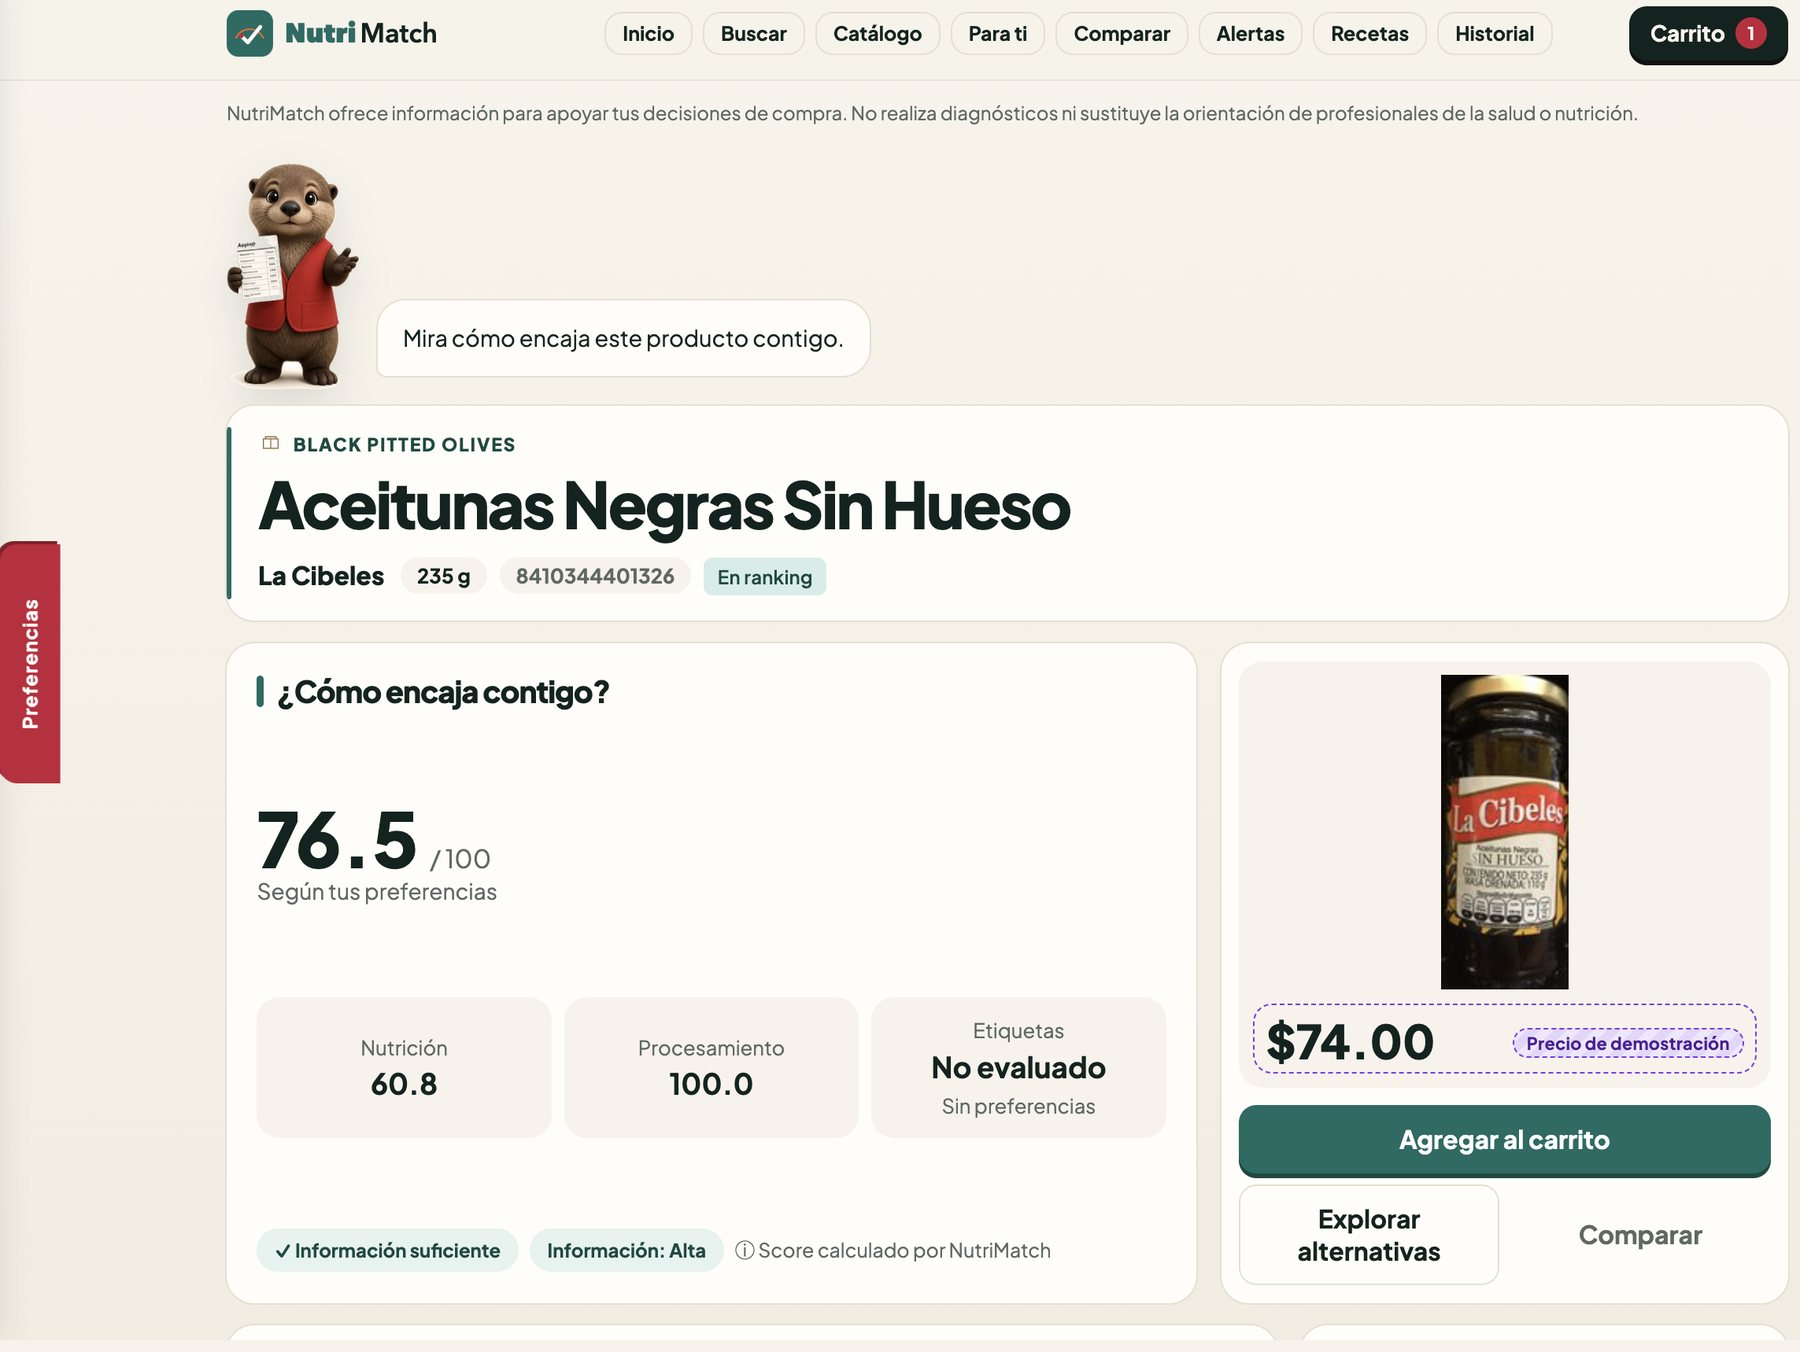
\includegraphics[width=\linewidth,height=62mm,keepaspectratio]{capturas/ficha-cibeles.jpg}\\[0.6mm]
      {\fine{La ficha muestra el resultado del motor. La pantalla redondea; el valor medido se cita en el caso.}}
    \end{column}
  \end{columns}
\end{frame}

% ---------- 10 ----------
\begin{frame}{De evaluar un producto a elegir una alternativa}
  \begin{columns}[T]
    \begin{column}{0.49\textwidth}
      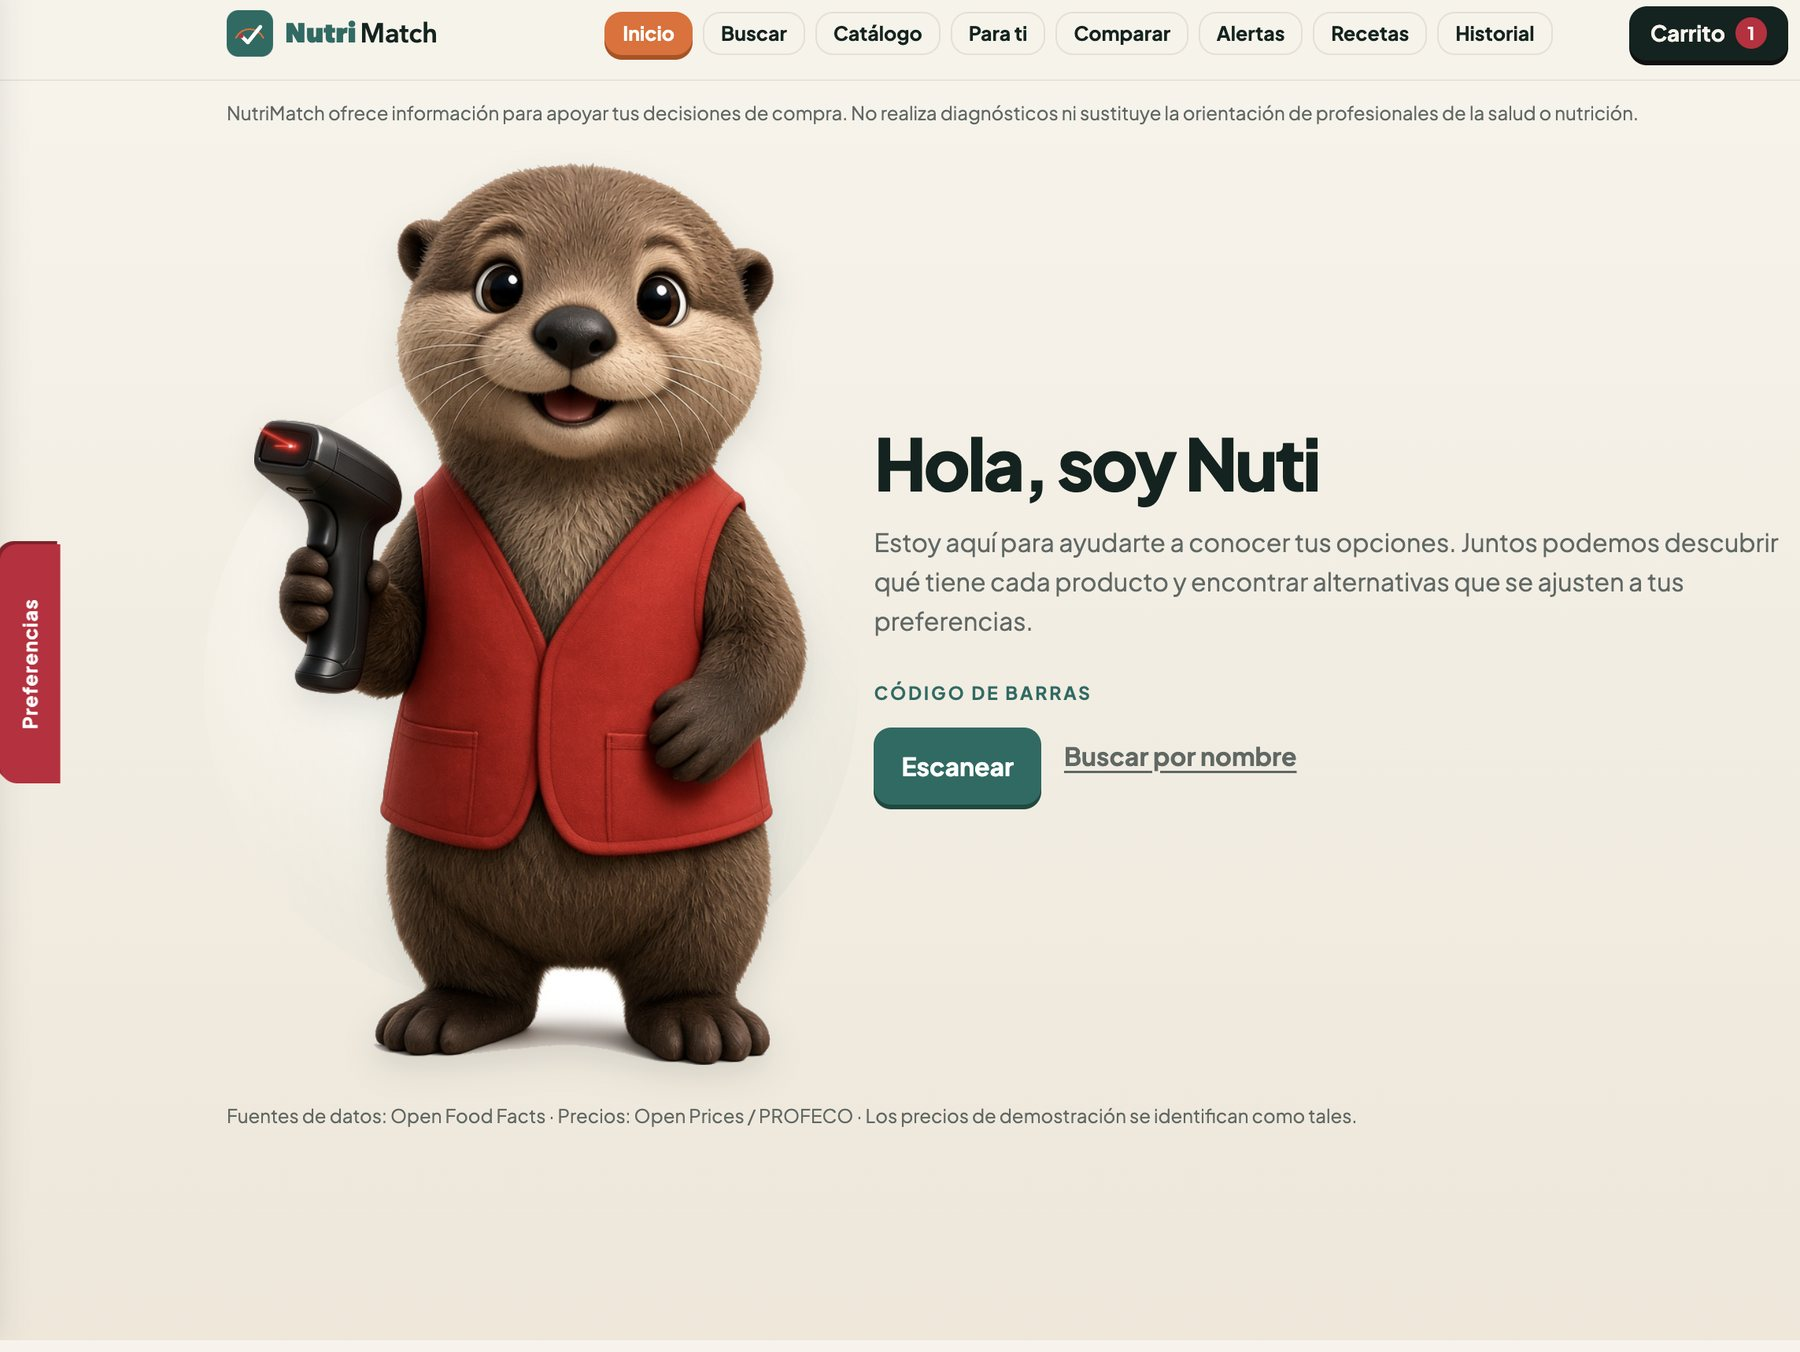
\includegraphics[width=\linewidth,height=26mm,keepaspectratio]{capturas/buscar.jpg}\\
      {\scriptsize\njsemibold\color{tide} Buscar}\\[0.8mm]
      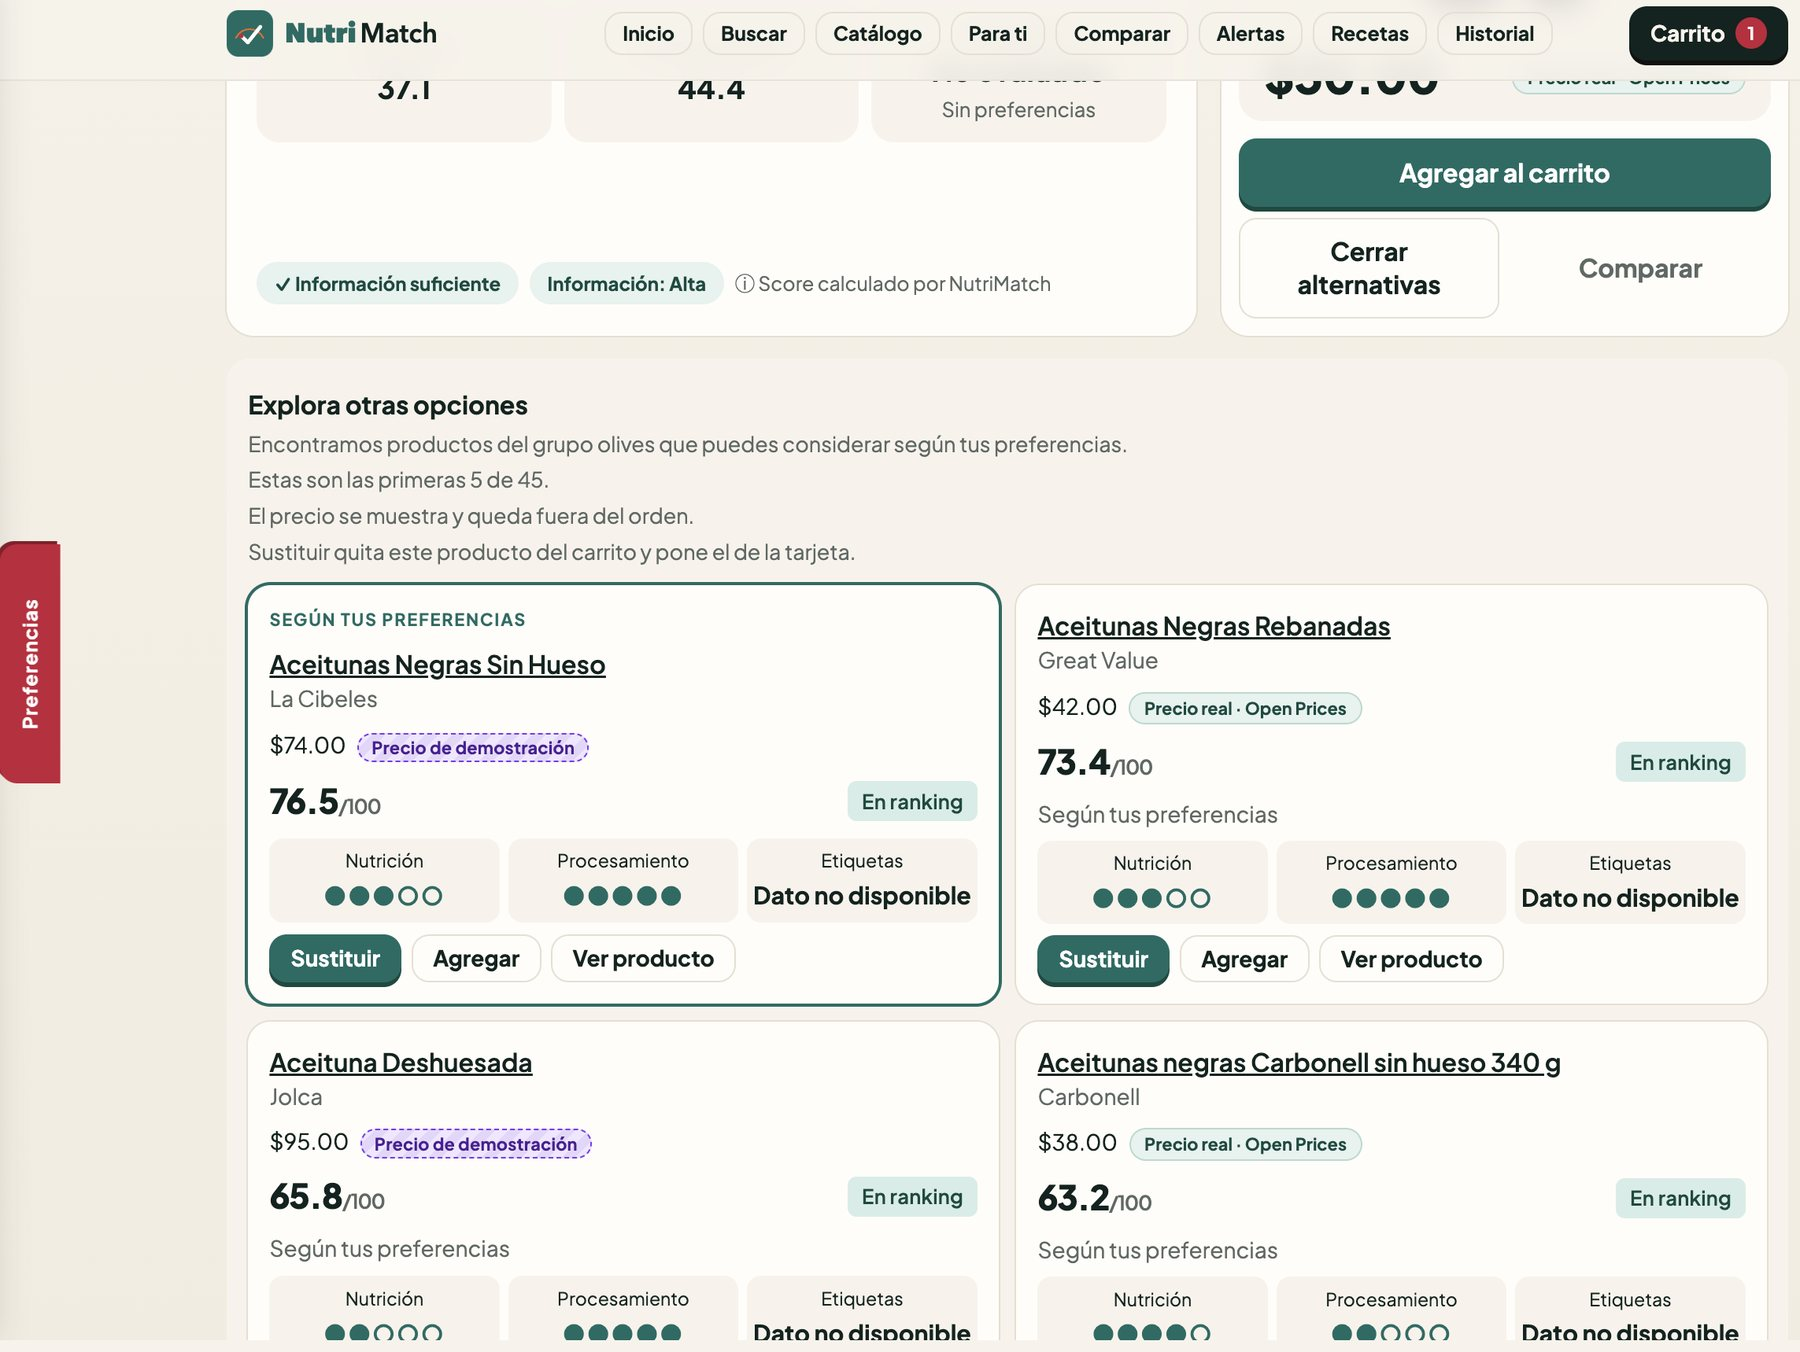
\includegraphics[width=\linewidth,height=26mm,keepaspectratio]{capturas/alternativas.jpg}\\
      {\scriptsize\njsemibold\color{tide} Sustituir}
    \end{column}
    \begin{column}{0.49\textwidth}
      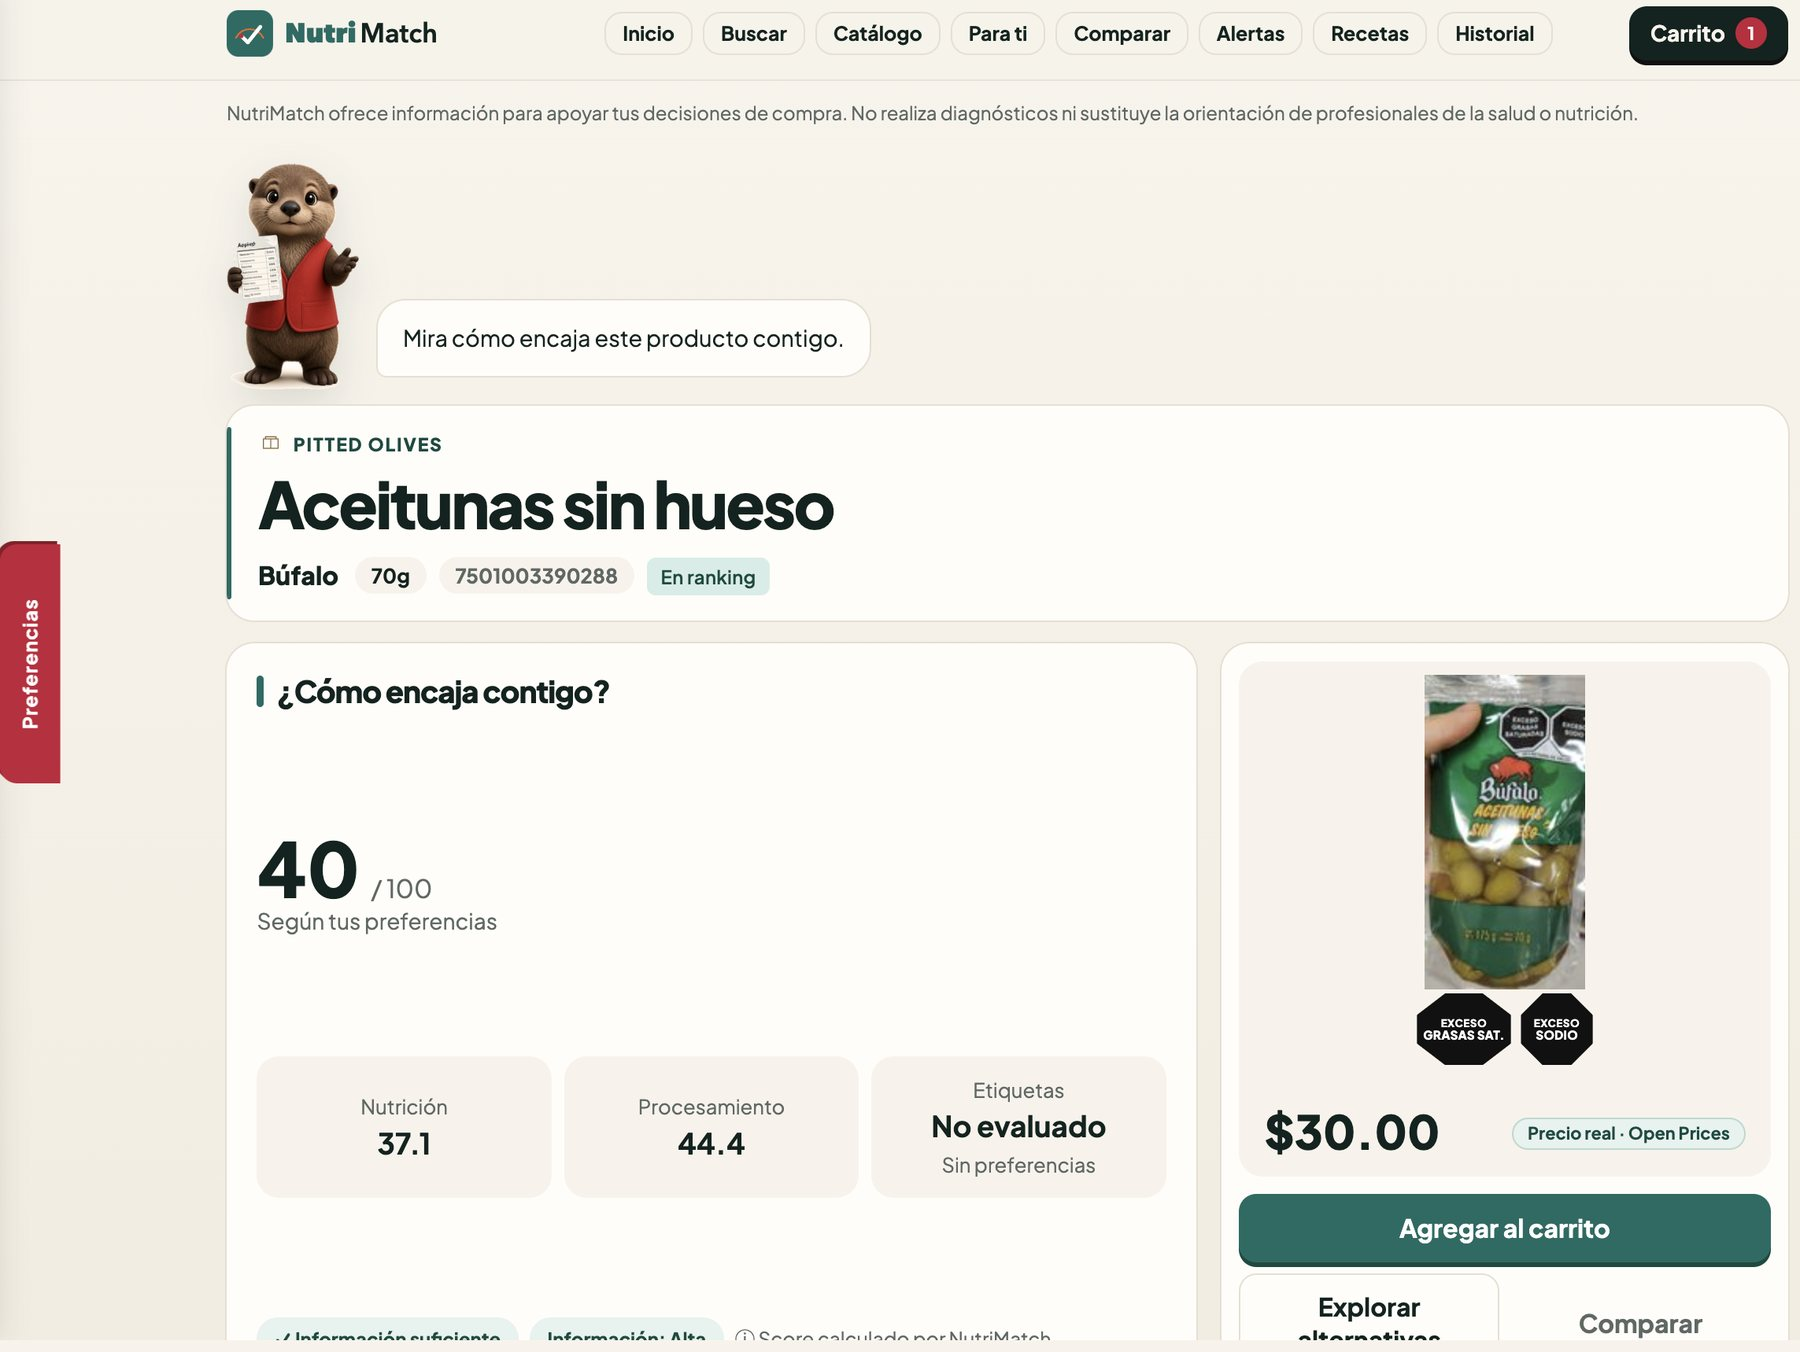
\includegraphics[width=\linewidth,height=26mm,keepaspectratio]{capturas/ficha-bufalo.jpg}\\
      {\scriptsize\njsemibold\color{tide} Evaluar}\\[0.8mm]
      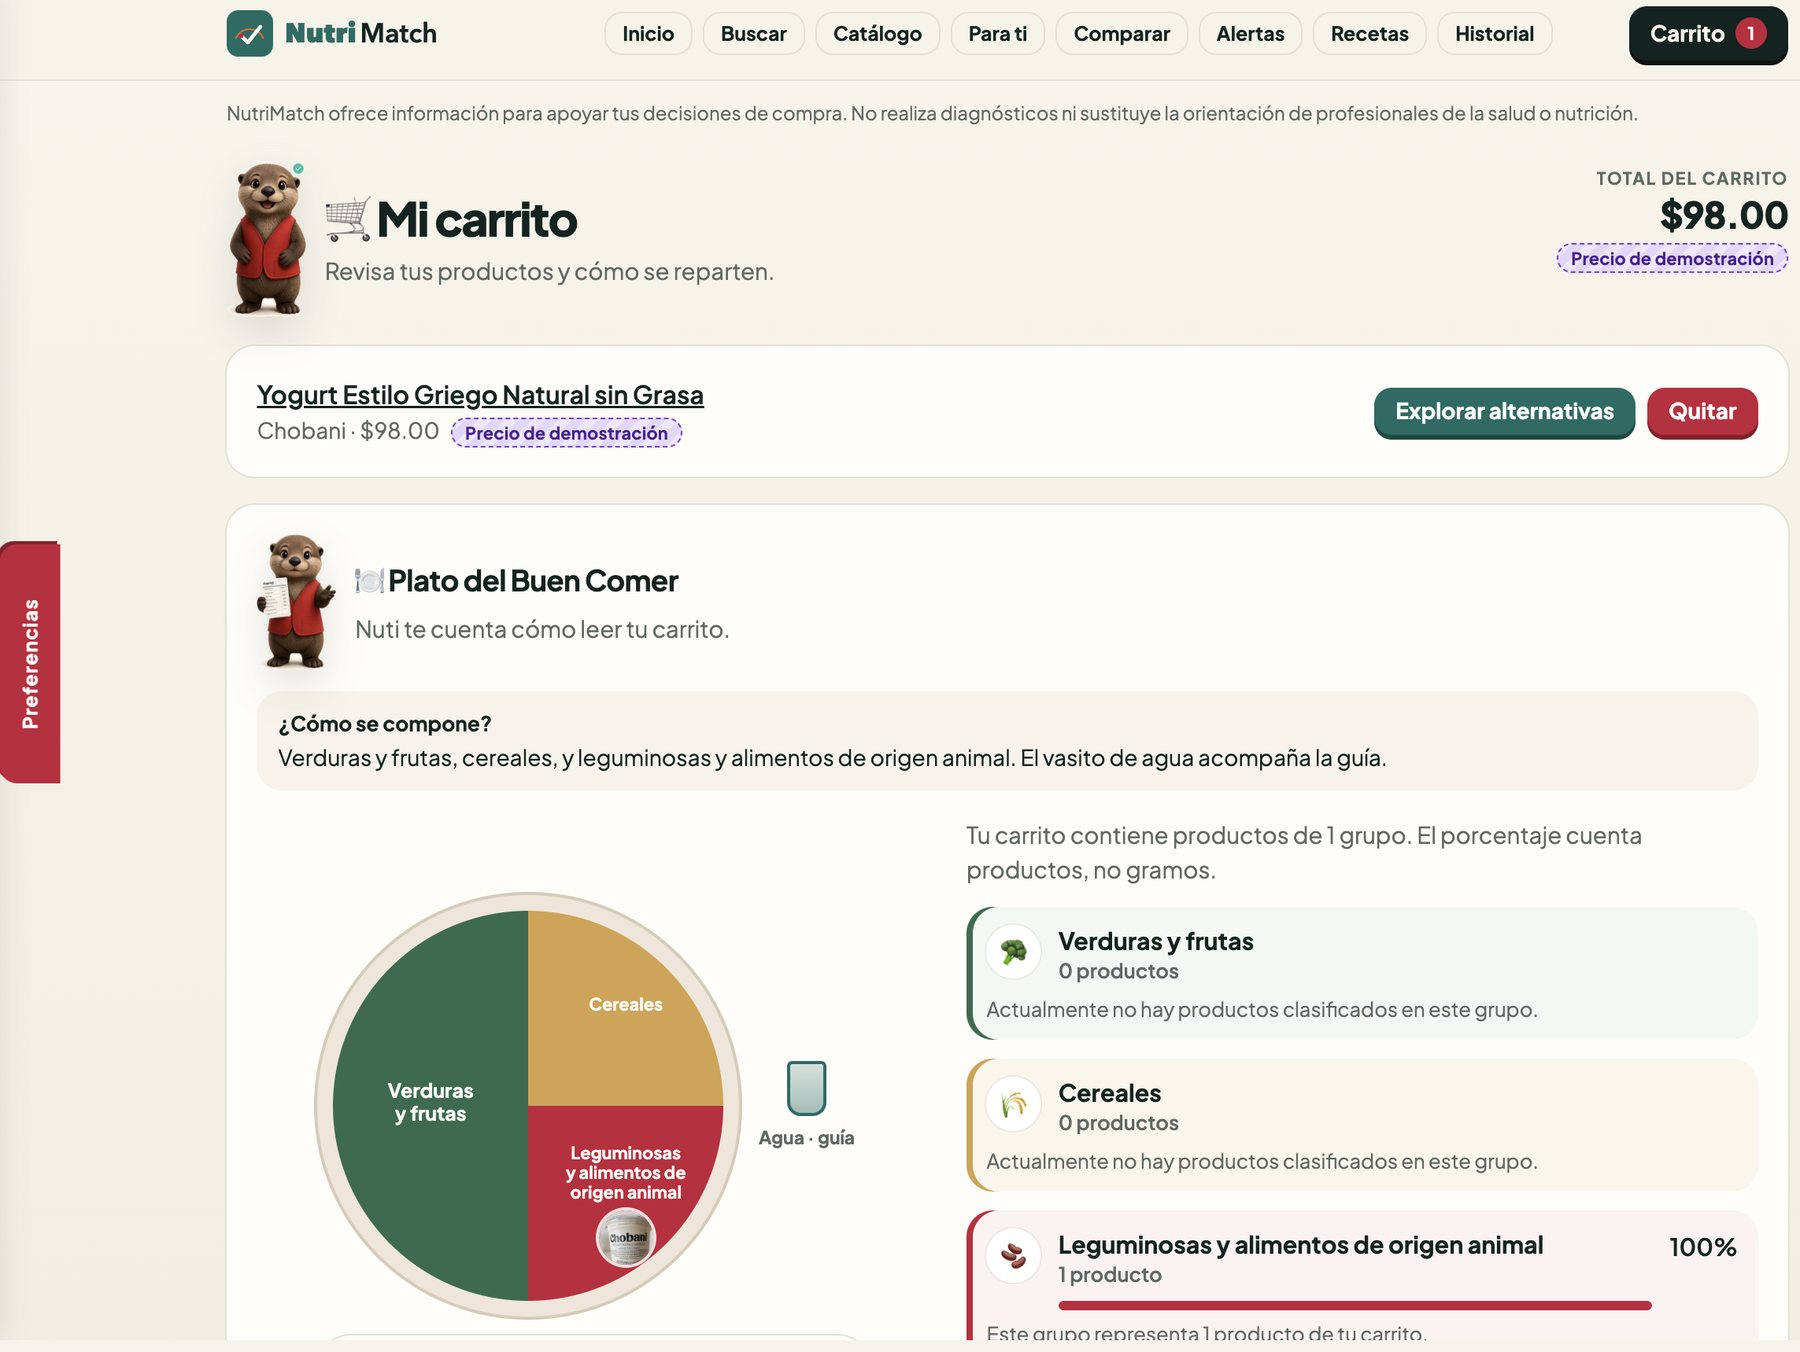
\includegraphics[width=\linewidth,height=26mm,keepaspectratio]{capturas/carrito.jpg}\\
      {\scriptsize\njsemibold\color{tide} Decidir}
    \end{column}
  \end{columns}
  \vspace{0.4mm}
  {\fine{Capturas de la aplicación en ejecución. El carrito es el que ya estaba guardado en el navegador; no es el caso de las aceitunas. El Plato del Buen Comer es el título de esa pantalla.}}
\end{frame}

% ---------- 11 ----------
\begin{frame}{Un ejemplo: elegir entre alternativas de la misma categoría}
  \card{\textwidth}{\scriptsize Perfil por defecto de la interfaz: nutrición, procesamiento y etiquetas, sin dieta y sin alérgenos. No es el perfil de 113 productos del cuaderno.}\par\vspace{1.2mm}
  \begin{columns}[T]
    \begin{column}{0.49\textwidth}
      {\scriptsize\color{tide}\njsemibold Producto consultado}\par\vspace{0.4mm}
      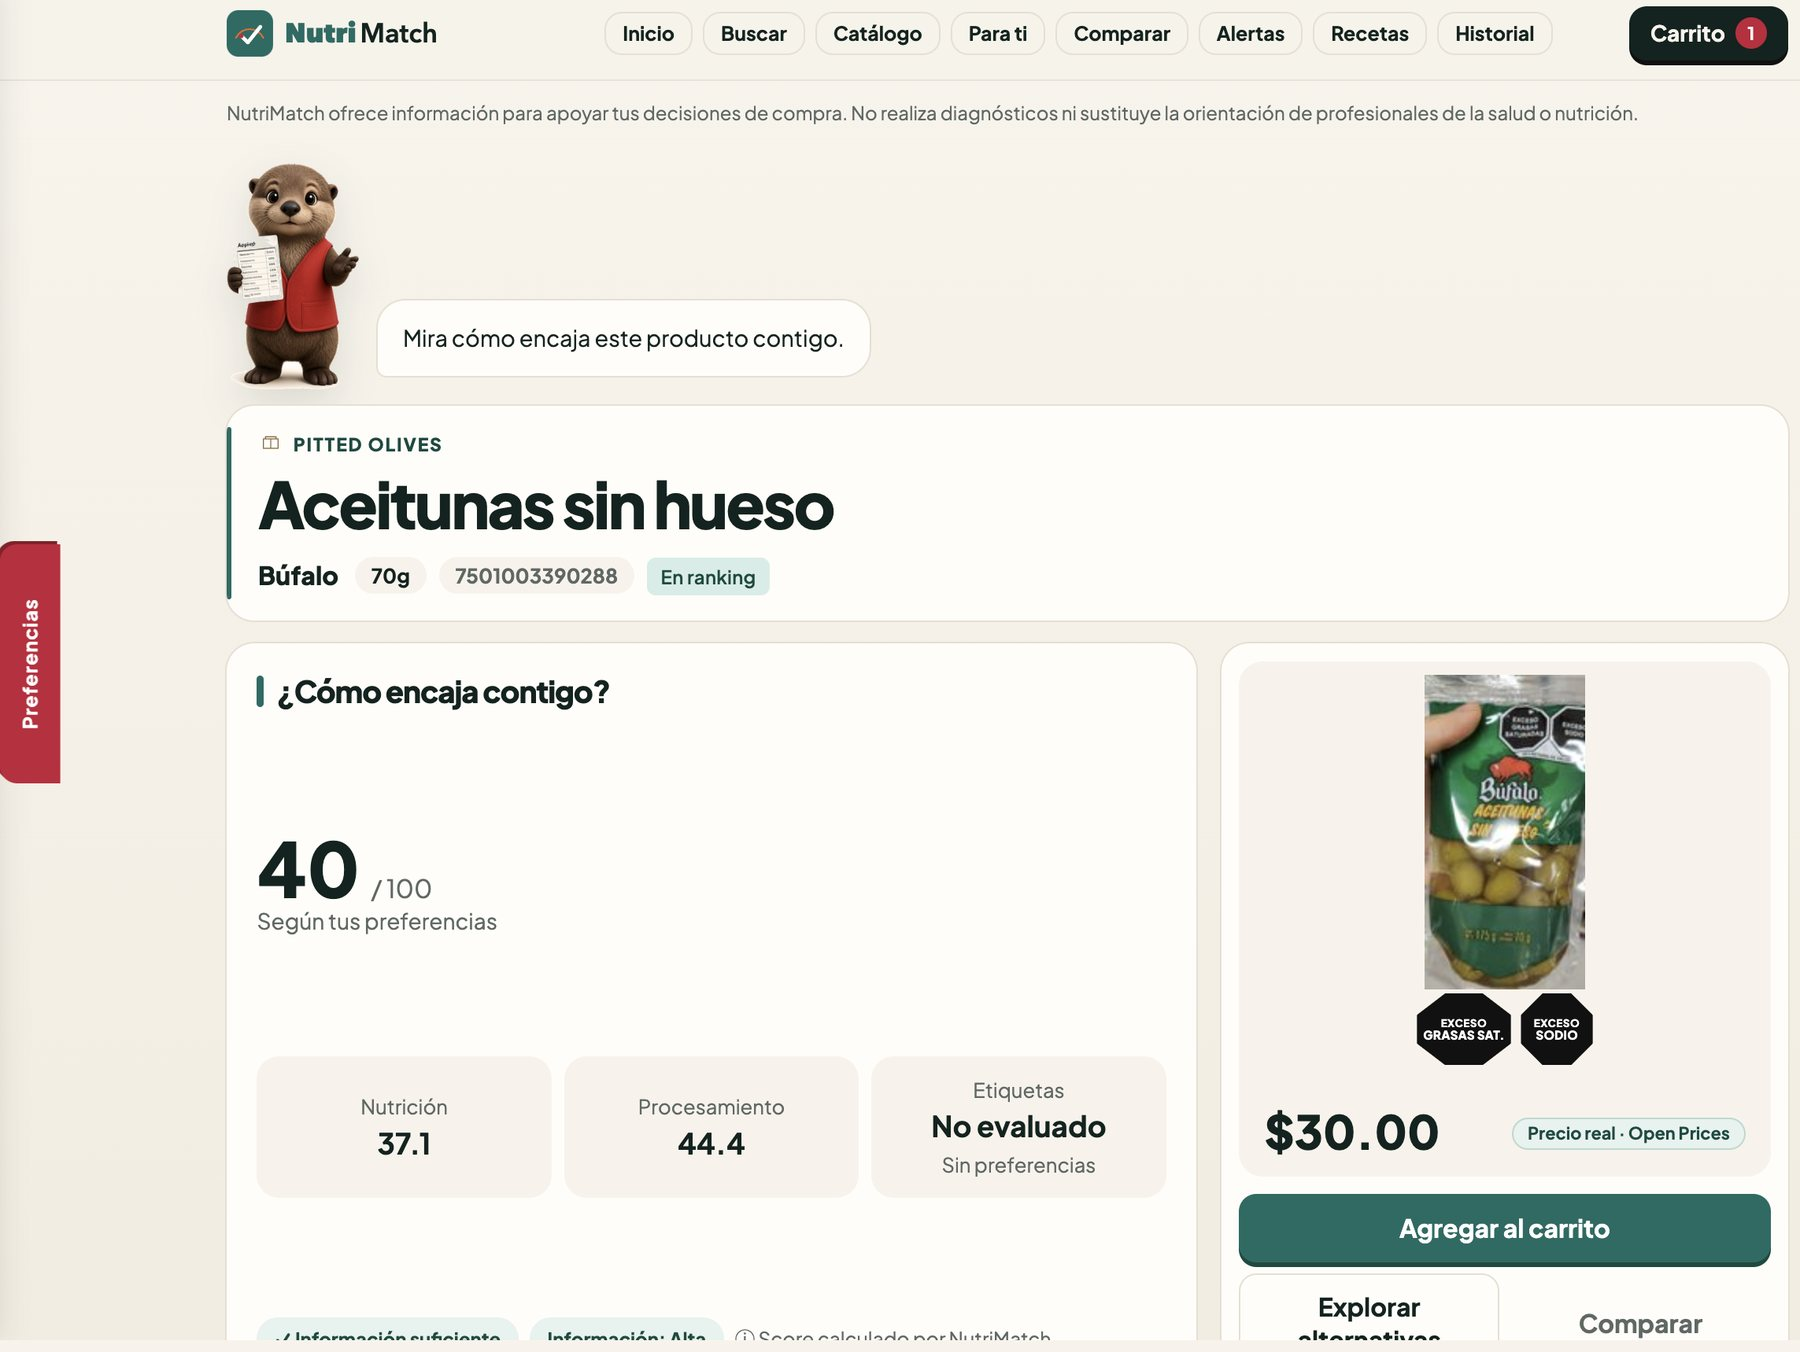
\includegraphics[width=\linewidth,height=30mm,keepaspectratio]{capturas/ficha-bufalo.jpg}\par\vspace{0.4mm}
      {\scriptsize 7501003390288 · Aceitunas sin hueso · Búfalo}\par
      {\metric{40,05}} {\scriptsize\quad \$30 precio real · NOVA 3 · sellos de exceso}\par
      {\fine{La pantalla muestra 40. El resultado medido es 40,05.}}
    \end{column}
    \begin{column}{0.49\textwidth}
      {\scriptsize\color{tide}\njsemibold Primera alternativa}\par\vspace{0.4mm}
      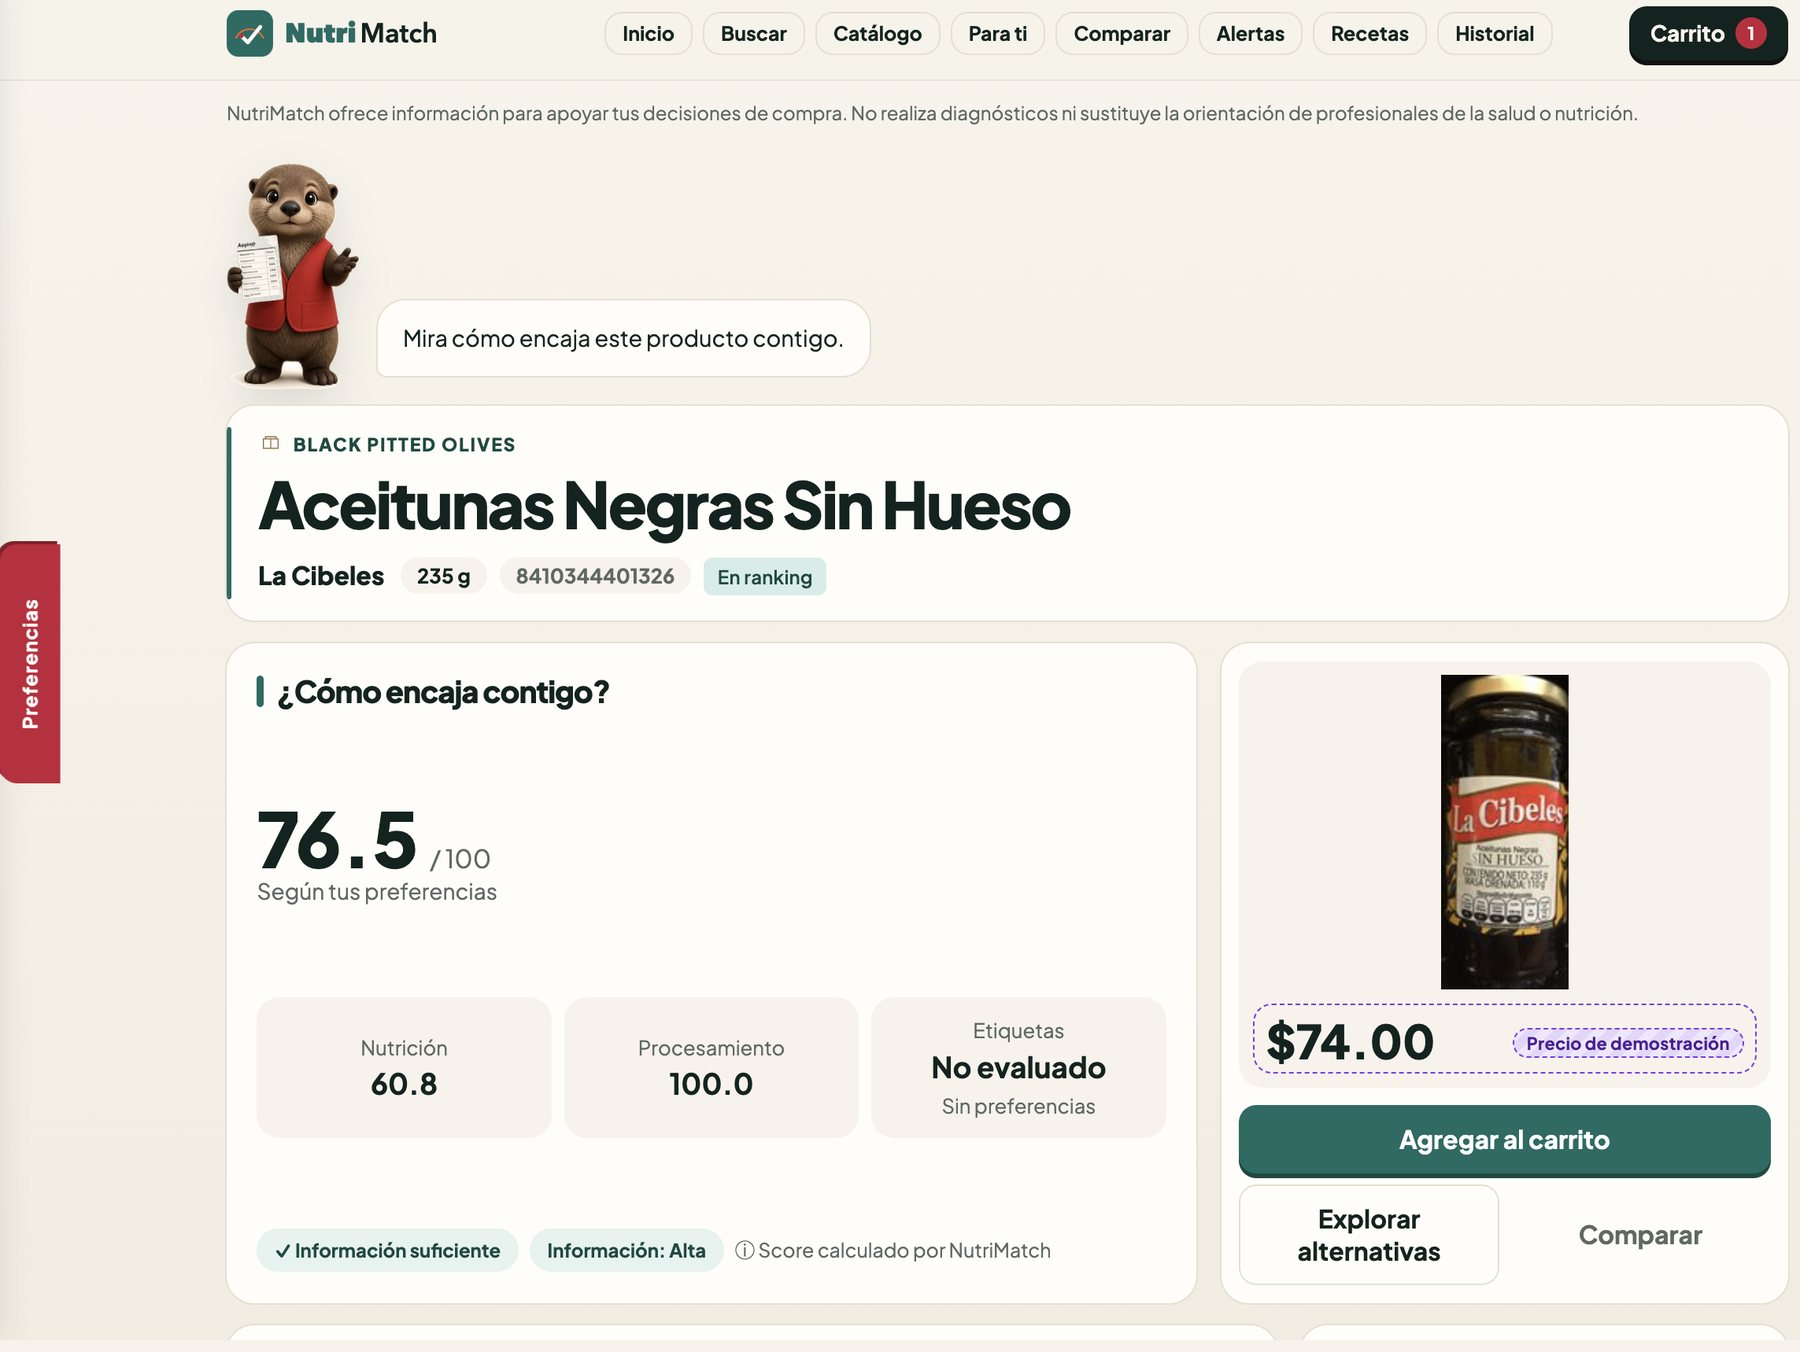
\includegraphics[width=\linewidth,height=30mm,keepaspectratio]{capturas/ficha-cibeles.jpg}\par\vspace{0.4mm}
      {\scriptsize 8410344401326 · Aceitunas negras sin hueso · La Cibeles}\par
      {\metric{76,48}} {\scriptsize\quad \$74 precio de demostración · NOVA 1}\par
      {\fine{La pantalla muestra 76,5. Los 74 pesos no están en el archivo y no ordenan.}}
    \end{column}
  \end{columns}
  \vspace{1mm}
  {\scriptsize Con este perfil, la alternativa obtiene una mayor puntuación.\par
  \njsemibold Una mayor puntuación no significa que el producto sea más saludable.}
\end{frame}

% ---------- 12 ----------
\begin{frame}[plain]
  \vspace{3mm}
  {\color{tide}\scriptsize\njsemibold CIERRE}\par\vspace{1mm}
  {\njextrabold\large De encontrar productos a elegir con información}\\[3mm]
  \begin{columns}[T]
    \begin{column}{0.32\textwidth}
      \card{\linewidth}{{\scriptsize\color{tide}\njsemibold Datos}\\[1mm]{\scriptsize 13\,093 productos integrados y caracterizados.}}
    \end{column}
    \begin{column}{0.32\textwidth}
      \card{\linewidth}{{\scriptsize\color{tide}\njsemibold Método}\\[1mm]{\scriptsize 5\,864 productos en el universo puntuable.}}
    \end{column}
    \begin{column}{0.32\textwidth}
      \card{\linewidth}{{\scriptsize\color{tide}\njsemibold Aplicación}\\[1mm]{\scriptsize Un motor reproducible conectado a una interfaz usable.}}
    \end{column}
  \end{columns}
  \vspace{3.5mm}
  \begin{columns}[c]
    \begin{column}{0.72\textwidth}
      {\njsemibold NutriMatch transforma un catálogo heterogéneo en información para decidir.}\\[1.5mm]
      {\color{mute} No decide por la persona qué alimento es saludable.}
    \end{column}
    \begin{column}{0.26\textwidth}
      
\includegraphics[width=\linewidth,height=28mm,keepaspectratio]{../../frontend/public/otter/nuti-recommend.png}
    \end{column}
  \end{columns}
\end{frame}

\end{document}
